\documentclass[border=10pt,tikz,multi]{standalone}
% \usetikzlibrary{shapes.geometric, positioning, arrows.meta}
\usetikzlibrary{positioning,shadows,arrows.meta,trees,shapes,fit}
\usepackage{fullpage}
\usepackage{calc}

\begin{document}

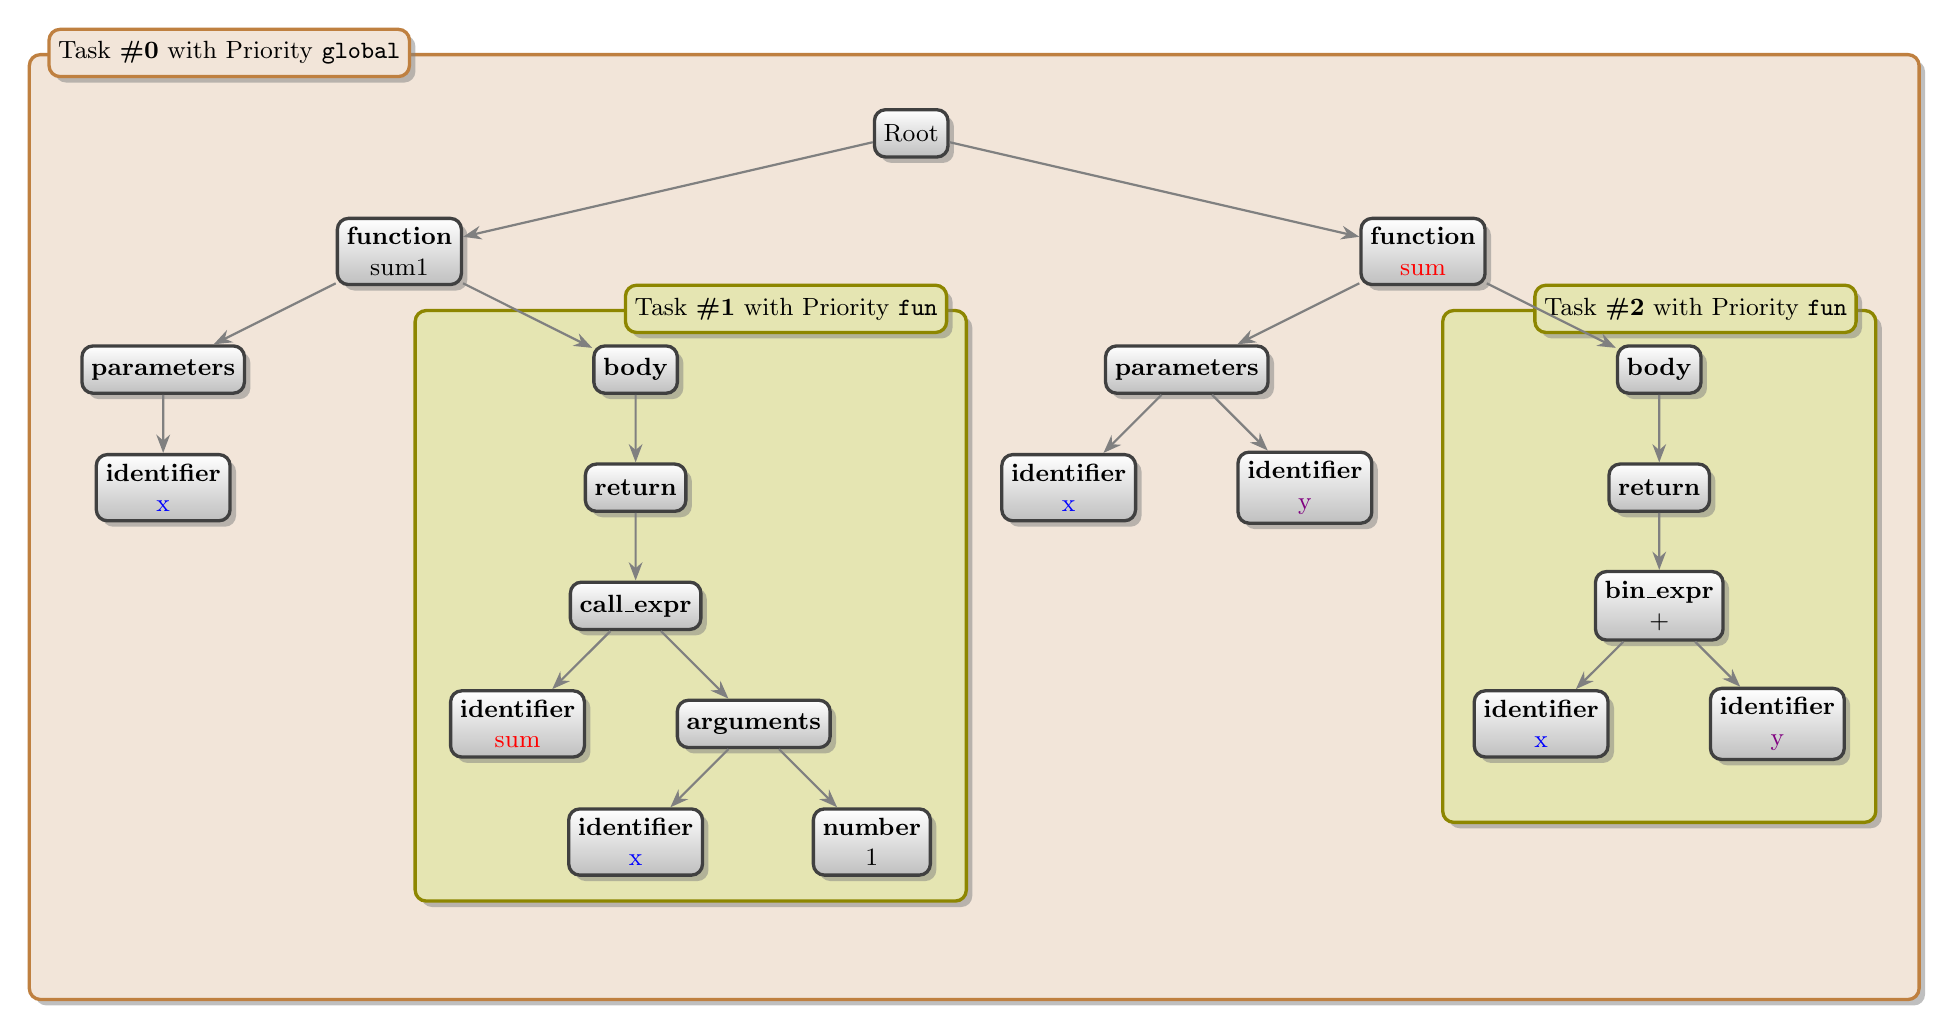
\begin{tikzpicture}
[font=\small, edge from parent,
    ->, >=Stealth,
    every node/.style={top color=white, bottom color=black!25,
        % fill=white,
    rectangle,rounded corners, minimum size=6mm, draw=black!75,
    very thick, drop shadow, align=center},
    edge from parent/.style={draw=black!50,thick},
    level 1/.style={sibling distance=13cm},
    level 2/.style={sibling distance=6cm},
    level 3/.style={sibling distance=3cm},
    level distance=1.5cm,
    ]
%     \node (A) {A}
%         child { node (B) {B}
%             child { node {B1}
%             edge from parent node[left=.5em,draw=none] {$\chi^2$} }
%             child { node {B2}}
%             }
%         child {node (C) {C}
%             child { node {C1}
%                 child { node {C1a}}
%             }
%         child { node {C2}}
%         child { node {C3}
%             child { node {C3a}}
%             child { node {C3b} edge from parent node[right=.5em,draw=none] {$\frac{a}{b}$}}
%             }
%         }
%     child { node {D}
%         child { node {D1}}
%         child { node {D2}}
% };

    % make a big rectangle
    \node[draw=brown,
          top color=brown!20,
          bottom color=brown!20,
          rectangle,
          very thick,
          rounded corners,
          fill=brown!20,
          minimum width=24cm,
          minimum height=12cm] (bigrect) at (0.8,-5) {};
    \node[draw=brown,text=black,
          top color=brown!20,
          bottom color=brown!20,
          right=0.25cm] at (bigrect.north west) {Task \textbf{\#0} with Priority \texttt{global}};


    \node[draw=olive,
          top color=olive!20,
          bottom color=olive!20,
          rectangle,
          very thick,
          rounded corners,
          fill=brown!20,
          minimum width=7cm,
          minimum height=7.5cm] (bigrect1) at (-2.8 ,-6) {};
    \node[draw=olive,text=black,
          top color=olive!20,
          bottom color=olive!20,
          left=0.25cm] at (bigrect1.north east) {Task \textbf{\#1} with Priority \texttt{fun}};

    \node[draw=olive,
          top color=olive!20,
          bottom color=olive!20,
          rectangle,
          very thick,
          rounded corners,
          fill=brown!20,
          minimum width=5.5cm,
          minimum height=6.5cm] (bigrect2) at (9.5 ,-5.5) {};
    \node[draw=olive,text=black,
          top color=olive!20,
          bottom color=olive!20,
          left=0.25cm] at (bigrect2.north east) {Task \textbf{\#2} with Priority \texttt{fun}};


    % \draw[dashed, very thick, rounded corners, anchor=north] (-9,1) rectangle (10.5,-10);
    % \draw[dashed, very thick, rounded corners, anchor=north] (-9,1) rectangle (10.5,-10)

    \node (root) {Root}
        child { node (sum1) {\textbf{function} \\ sum1}
            child { node {\textbf{parameters}}
              child { node {\textbf{identifier} \\ \textcolor{blue}{x}} }
            }
            % edge from parent node[left=.5em,draw=none] {$\chi^2$} }
            child { node {\textbf{body}}
              child { node {\textbf{return}}
                child { node {\textbf{call\_expr}}
                  child { node {\textbf{identifier} \\ \textcolor{red}{sum}} }
                  child { node {\textbf{arguments}}
                    child { node {\textbf{identifier} \\ \textcolor{blue}{x}} }
                    child { node {\textbf{number} \\ 1} }
                  }
                }
              }
           }
        }
        child { node (sum1) {\textbf{function} \\ \textcolor{red}{sum}}
            child { node {\textbf{parameters}}
              child { node {\textbf{identifier} \\ \textcolor{blue}{x}} }
              child { node {\textbf{identifier} \\ \textcolor{violet}{y}} }
            }
            % edge from parent node[left=.5em,draw=none] {$\chi^2$} }
            child { node {\textbf{body}}
              child { node {\textbf{return}}
                child { node {\textbf{bin\_expr} \\ +}
                    child { node {\textbf{identifier} \\ \textcolor{blue}{x}} }
                    child { node {\textbf{identifier} \\ \textcolor{violet}{y}} }
                }
              }
           }
        };

\end{tikzpicture}

\end{document}
